\def\problemset#1#2#3{
\noindent\rule{16.5cm}{1pt}
\begin{center}
  \parbox{16.5cm}{\bf
    STAT 598Z Homework 5 \\
    Instructor: Prof. S V N Vishwanathan \hfill Jiajie Huang\\
    Due April 2nd, 2013 \hfill huang147@purdue.edu
    }
\end{center}
\noindent\rule{16.5cm}{0.5pt}
}

\newcommand{\lb}[1]{\left \lfloor #1 \right \rfloor}
\newcommand{\bmat}[1]{\begin{bmatrix} #1 \end{bmatrix}}
\documentclass[fleqn, 11pt]{article}
\usepackage{fullpage}
\usepackage{hyperref}
\usepackage{ulem}
\usepackage{amsmath}
\usepackage{algorithm}
%\usepackage{algorithmic}
\usepackage{algpseudocode}
\setlength{\parindent}{0in}
\usepackage{graphics}
\usepackage{graphicx}
\usepackage{mathtools}


\begin{document}

\problemset{3}{Problem Set 2}{\today}


\section*{Problem 1}

\begin{itemize}
\item The data points in the three classes don't have any covariance in their two dimensions, which makes the sample generation much easier. For example, for class $1$, $mean=(0,0)$, $covariance$ $matrix$ $= I$, I just simply draw random samples in each dimension with $mean = 0$ and $standard$ $deviation$ $= 1$, then combine the two samples as one. Repeat the steps above for each class and get all three classes of samples. See the plot of sample points in Figure \ref{three} below (blue for class $1$, red for class $2$, green for class $3$). 

\begin{figure}[htb]
\centering
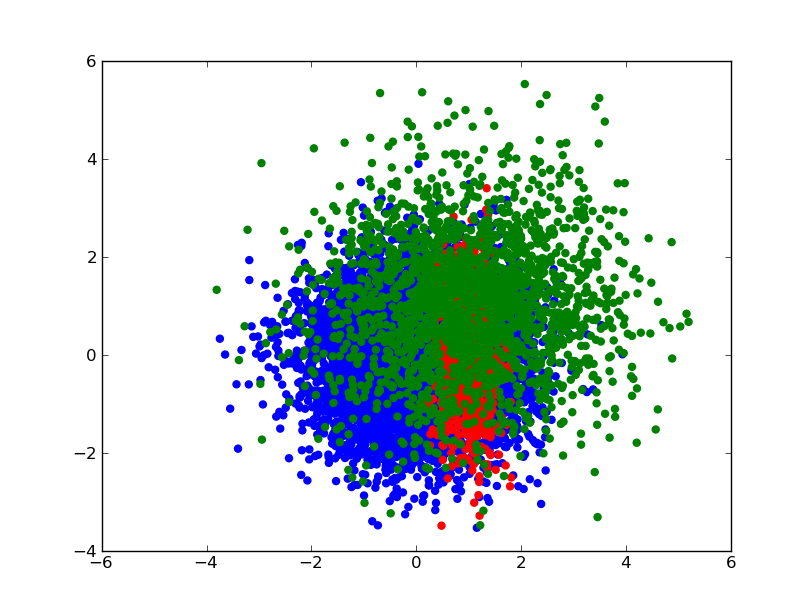
\includegraphics[width=18cm]{hw5.png}
\caption{Plot of three classes of samples: class $1$ as blue, class $2$ as red, class $3$ as green }
\label{three}
\end{figure}

\item I implemented a $k$ nearest neighbors classifier using $k=1$ here. The distance function for two points $A(x_1,y_1)$ and $B(x_2,y_2)$ is:
\[
d(A(x_1,y_1),B(x_2,y_2))=\sqrt{(x_1-x_2)^2+(y_1-y_2)^2}
\]
For my code, I used matrix computation to simplify the calculation. For each point $A$ in test data, I calculate an array of distances, which are the distances of $A$ and all the points $B_i$ ($i=1...n$, $n$ is the number of points in training data) in the training data. Then for each array of distances, get the minimum distance $d(A,B_i)$ and find $label_A$ as label of $A$, and $label_{B_i}$ as label of $B_i$. Compare labels, if $label_A = label_{B_i}$, then the prediction is correct; otherwise prediction is incorrect. Calculate the correctness for all the points in test data and get a accuracy based on the counts of total correct points $n_C$ and total incorrect points $n_{IC}$:
\[
Accuracy = \frac{n_C}{n_C+n_{IC}}
\]
Using group $1,2,3$ for three groups of test data, respectively, and group $0$ for all the three groups of test data, the accuracy for my classifier when $k=1$ is 
\begin{verbatim}
test group=0,k=1,correct rate=0.52
test group=1,k=1,correct rate=0.80
test group=2,k=1,correct rate=0.34
test group=3,k=1,correct rate=0.41
\end{verbatim}


\item When generalize $k$ to larger numbers, here I use $k=1$ to $5$. The algorithm is similar to the one above ($k=1$), but I need to modify the part of predicting point $A$ based on a list of $k$ minimum distances. So for each point $A$ in test data, I first sort the distance array, then get the first $k$ distances $d(A,B_k)$, then find out the labels for point $B_k$ (here $k= 1$ to $5$), then find out the label with the maximum count, which is used as the predicted label for point $A$. Something I need to point out is, when there are more than 2 labels with the same count and that count is maximum, just randomly pick one label as the predicted label; however, if we need to do this more accurately we need to give weights to different distances and rank the labels by modified distances. 

My result using my knn classifier is as below:
\begin{verbatim}
test group=0,k=2,correct rate=0.53
test group=1,k=2,correct rate=0.73
test group=2,k=2,correct rate=0.38
test group=3,k=2,correct rate=0.41
 
test group=0,k=3,correct rate=0.50
test group=1,k=3,correct rate=0.66
test group=2,k=3,correct rate=0.28
test group=3,k=3,correct rate=0.47
 
test group=0,k=4,correct rate=0.51
test group=1,k=4,correct rate=0.70
test group=2,k=4,correct rate=0.33
test group=3,k=4,correct rate=0.41
 
test group=0,k=5,correct rate=0.55
test group=1,k=5,correct rate=0.72
test group=2,k=5,correct rate=0.34
test group=3,k=5,correct rate=0.45
\end{verbatim}

What I find out is:
\begin{itemize}
\item The accuracy largely depends on the size of training data sets. Sample $2$ has least points (only $1,000$, or $10\%$ of total training data points) of the whole training set, so its affect on classifying the test data points is overwhelmed by training points from the other two sets, therefore it has a smallest accuracy in classifying test points. Sample $3$ has a similar situation as sample $2$ here. Sample $1$ has a largest sample size ($7,000$, or $70\%$ of data points), so it is not so badly affected by other samples and thus has a largest accuracy (around $0.7$).  

\item The accuracy also depends on the distribution of different training sets. Sample $2$ is distributed between sample $1$ and $3$ (with its mean between sample $1$ and $3$) so it can easily mix up with the other two; and moreover, sample $3$ has a larger variation (a larger standard deviation in both $x$ and $y$ axis) than the other two samples, so the points in sample $3$ can also easily mess up with the points in sample $2$. 

\item To sum up, if we want an accurate result, our training data sets should be well separated. As we can see from the plot on Figure \ref{three}, the three training data sets are so closely to each other that at some parts they are even overlapping, and we can not tell them apart from our eyes. Given such a messy training set it is hard to use them to classify test data sets. 
\end{itemize}

\item When $k>1$, for classifying one point in test set, an array of distance is calculated using python linear algebra method, which is considered as $O(d)$ effort because it is well optimized in python and only related to the dimension of data. For sorting the array and get the minimum $k$ distances (I use $numpy.sort$ function here), complexity is $O(n_1\log(n_1))$. Finding the label with maximum count in $k$ neighbors, complexity is $O(k)$. So complexity of classifying one point in the test set is $O(d*n_1*\log(n_1)*k)=O(dkn_1\log(n_1))$. For classifying the total test set of $n_2$ points, the complexity is $O(n_2*dkn_1\log(n_1))=O(dkn_1n_2\log(n_1))$. If we consider the dimension of data $d$ and the number nearest neighbors $k$ as constants, then the total complexity is bound at $n_1n_2\log(n_1)$, i.e. the total complexity is $O(n_1n_2\log(n_1))$, which only depends on the size of test and training data sets. But for large data sets with large dimensions $d$ (lots of features), we can not ignore $d$ in the complexity, so the complexity would be at least $O(dn_1n_2\log(n_1))$. 

For $k=1$, everything is the same except the part for finding the minimum distance in the distance array, where I use a python function called $argmin$ to find out the minimum distance. If only loop over the array and find the minimum, the complexity is $O(n_1)$ here. So the total complexity is $O(dkn_1n_2)=O(dn_1n_2)$. 

\item I use $dna.scale$ and $dna.scale.t$ in $dna$ data set for training and testing, respectively. There are $3$ classes and $180$ features (dimensions) in the data, with $2,000$ rows and $1,186$ rows in training and testing data, respectively. I wrote two python functions $def$ $read$ and $def$ $insertvalue$ to read in the raw data files ($.txt$ format) and make them the same format as the normal distribution data points before. I use the same $knn$ classifier I wrote to do classification: 

\begin{verbatim}
k=1,correct rate=0.77
k=2,correct rate=0.75
k=3,correct rate=0.75
k=4,correct rate=0.75
k=5,correct rate=0.75
\end{verbatim}

So the accuracy is above $0.75$ for all $k=1$ to $5$, which is much better than that of the normal distribution problem we just did above. That means the training data points should be much better separated in space (however, they are high dimensional here, with $d=180$ and can not be plotted for a better view). 

\end{itemize}





\end{document}